\documentclass[../report.tex]{subfiles}

\begin{document}

\graphicspath{{img/}{../img/}}

\section{Scrum men... Ikke helt}
\label{sec:Scrum}


\paragraph{Hvad er Scrum?}
Scrum er en agil software udviklings metode, hvis hovedm�l er h�ndteringen af l�bende �ndringer i kravspecifikationen. Indenfor h�ndtering af �ndringer er Scrum's mods�tning vandfaldsmodellen, som ikke tager sig p�nt i et milj� men mange krav�ndringer.

\paragraph{Scrum men... Hvad mangler s�?}
I target-projektet bliver der arbejdet efter Scrum, men ikke Scrum i dets fulde forstand. Det blev besluttet at k�re l�st p� nogle af Scrums discipliner, fordi der var enighed om at det ikke gav meget mening for en projektgruppe der kun m�des et par gange om ugen. Se figur \ref{fig:Scrum} p� side \pageref{fig:Scrum} \\

\begin{figure}[H]
\centering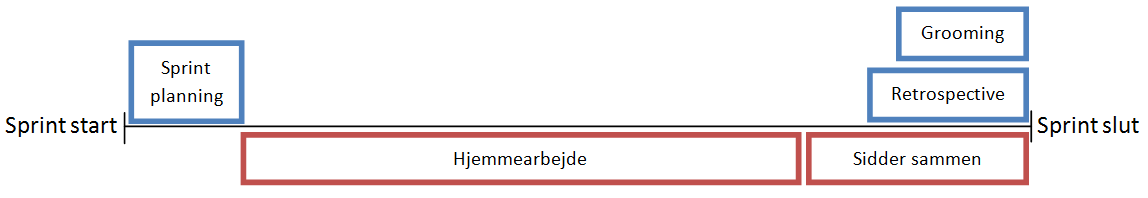
\includegraphics[scale=0.45]{SCRUMtimeLine.png}
\caption{Sprint tidslinje}
\end{figure}

\begin{figure}
\begin{tabularx}{14cm}{c|X}
\textbf{Aktiviteter}  & \textbf{Beskrivelse} \\
Scrum roller & I et eksamensprojekt er det urealistisk at have en person til kun at v�re product owner. I target-projektet er product owner ene og alene ansvarlig for kommunikation med stakeholders og prioritering af product items, men han er ogs� udvikler i Scrum teamet. Derudover er Scrummaster og developers blevet brugt klassisk.     \\ 
 & \\
Standup meeting & Der blev ikke afholdt nogen standup meetings \\
 & \\
Grooming & Den n�stsidste aktivitet var grooming, hvor Scrumboardet bliver rydtet op. \\
 & \\
Retrospective & Den sidste aktivitet var retrospective. Gruppen benyttede Keep-Stop-New metoden\footnote{http://www.mountaingoatsoftware.com/agile/scrum/sprint-retrospective/}. \\
 & \\
Sprint planning & Den f�rste aktivitet i hvert sprint er en klassisk sprint planning \\
 & \\
Scrumboard & Scrum boardet er den centrale oversigt over aktiviteter. Da target-projektgruppen ikke havde et fast lokale allokeret, var et fysisk Scrumboard ikke muligt, s� online v�rkt�jet Trello\footnote{Trello.com} bliver brugt i stedet \\
 & \\
Tidstagning & Der blev i fire sprints taget tid p� arbejdet med Toggl\footnote{Toggl.com}\\
 & \\
\end{tabularx}
\label{fig:Scrum}
\caption{Target-projektets aktiviteter}
\end{figure} 

\todo mere omkr. hvad vi har pr�vet

\end{document}